\section{Postgres-X2}
\label{sec:postgres-x2}

Postgres-X2~-- система для создания мульти-мастер кластеров, работающих в синхронном режиме~-- все узлы всегда содержат актуальные данные. Postgres-X2 поддерживает опции для увеличения масштабирования кластера как при преобладании операций записи, так и при основной нагрузке на чтение данных: поддерживается выполнение транзакций с распараллеливанием на несколько узлов, за целостностью транзакций в пределах всего кластера отвечает специальный узел GTM (Global Transaction Manager).

Измерение производительности показало, что КПД кластера Postgres-X2 составляет примерно 64\%, т.е. кластер из 10 серверов позволяет добиться увеличения производительности системы в целом в 6.4 раза, относительно производительности одного сервера (цифры приблизительные).

Система не использует в своей работе триггеры и представляет собой набор дополнений и патчей к PostgreSQL, дающих возможность в прозрачном режиме обеспечить работу в кластере стандартных приложений, без их дополнительной модификации и адаптации (полная совместимость с PostgreSQL API). Кластер состоит из одного управляющего узла (GTM), предоставляющего информацию о состоянии транзакций, и произвольного набора рабочих узлов, каждый из которых в свою очередь состоит из координатора и обработчика данных (обычно эти элементы реализуются на одном сервере, но могут быть и разделены).

Хоть Postgres-X2 и выглядит похожим на MultiMaster, но он им не является. Все сервера кластера должны быть соединены сетью с минимальными задержками, никакое географически-распределенное решение с разумной производительностью построить на нем невозможно (это важный момент).

\subsection{Архитектура}

\begin{figure}[ht!]
  \center{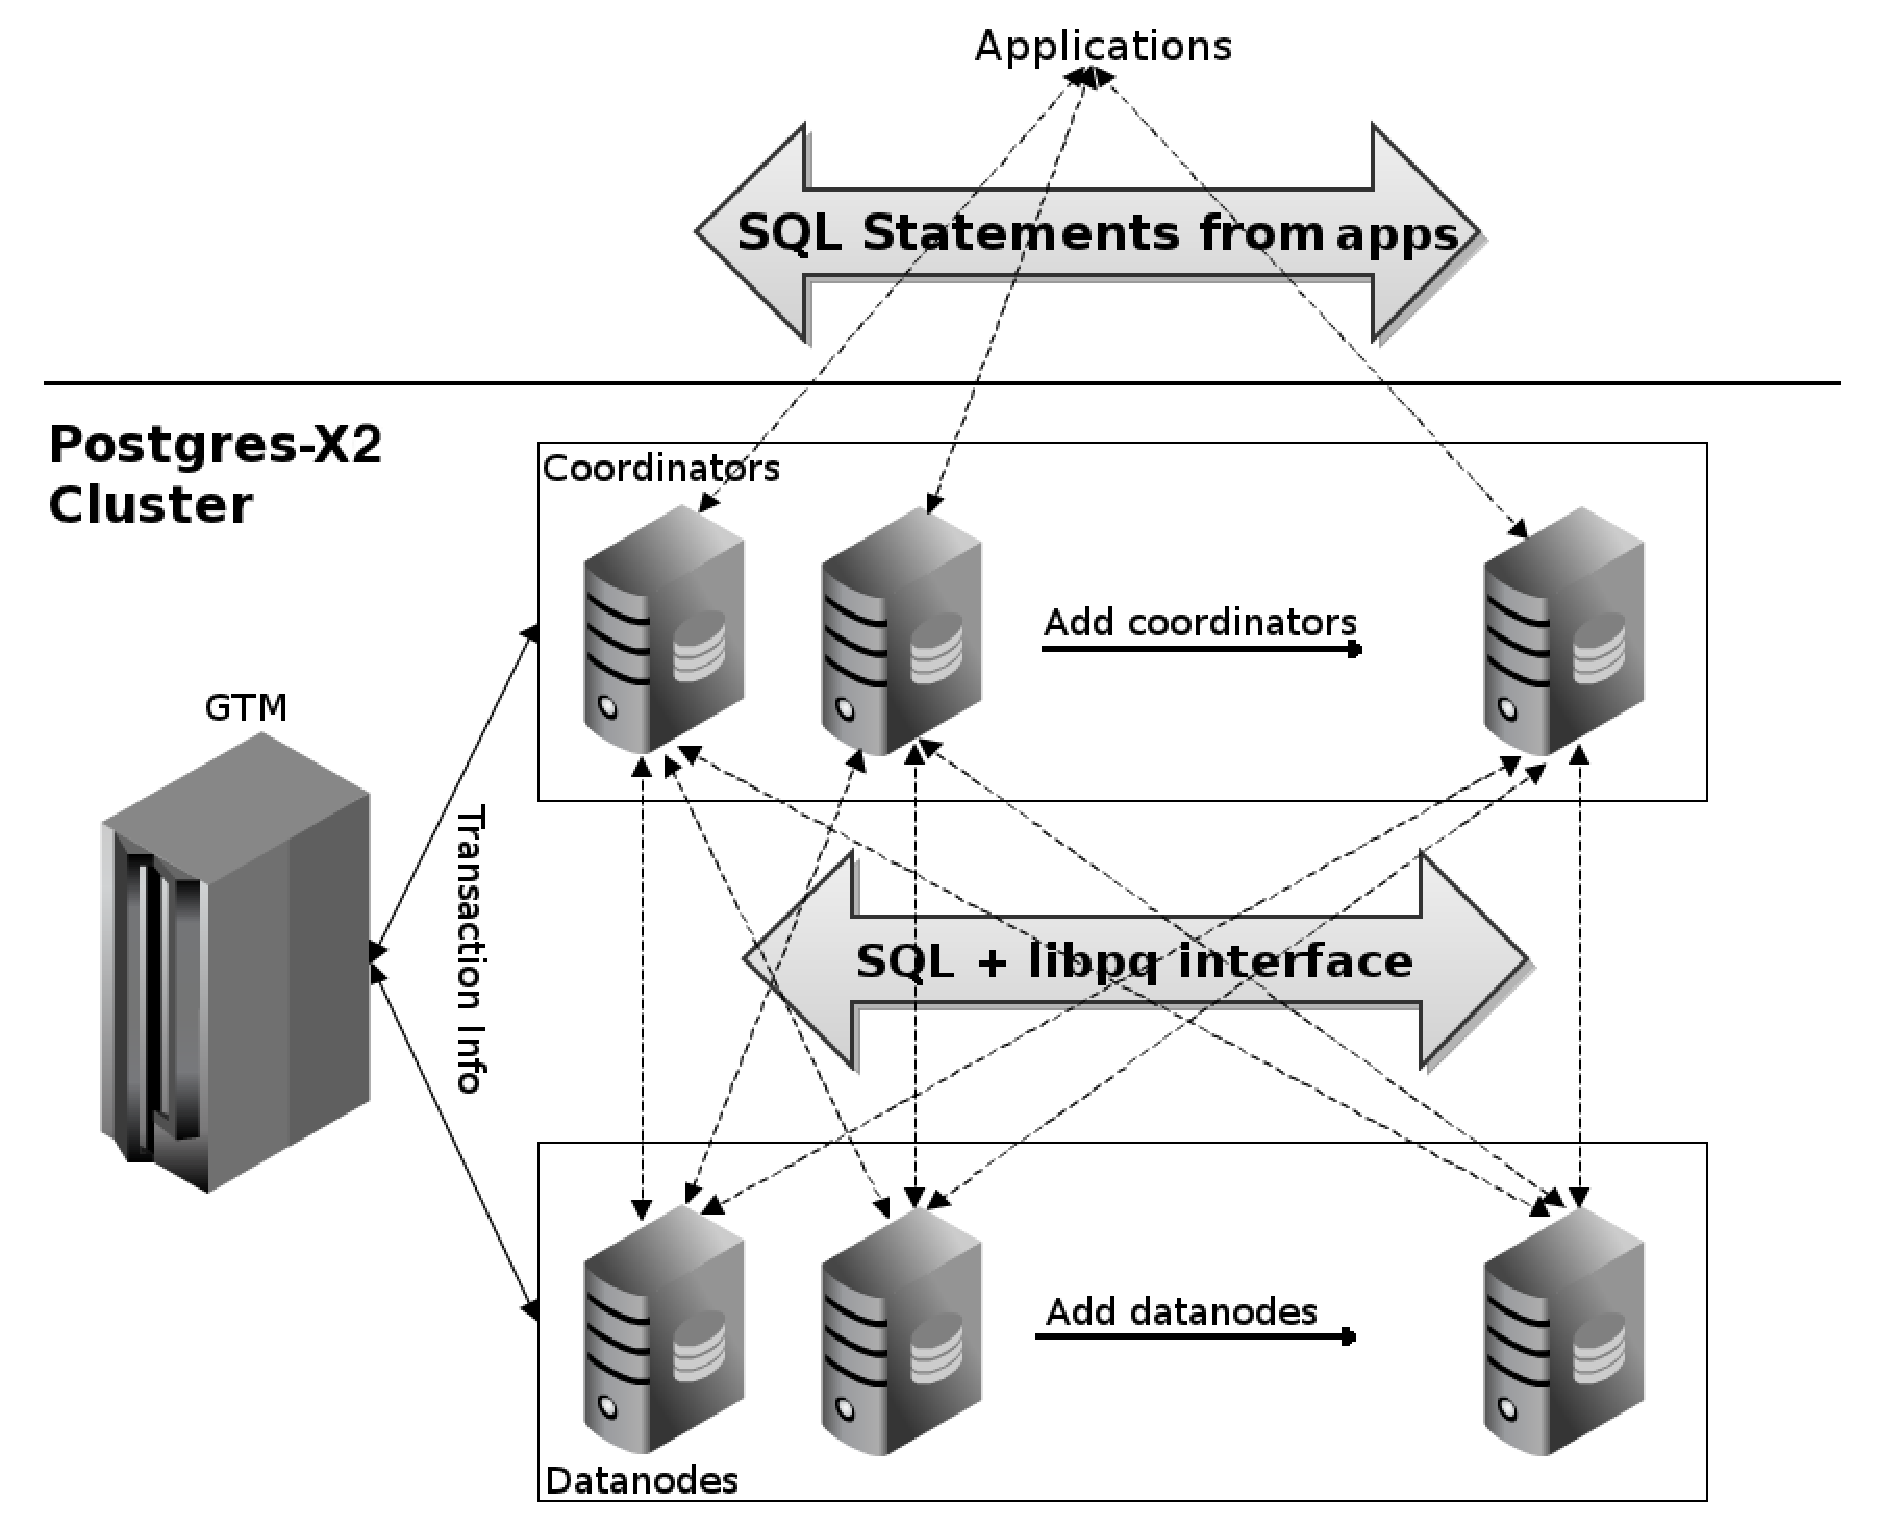
\includegraphics[width=1\textwidth]{postgres-x2-arch.pdf}}
  \caption{Архитектура Postgres-X2}
  \label{fig:postgres-x21}
\end{figure}

Рис.~\ref{fig:postgres-x21} показывает архитектуру Postgres-X2 с тремя её основными компонентами:

\begin{enumerate}
  \item Глобальный менеджер транзакций (GTM)~--- собирает и обрабатывает информацию о транзакциях в Postgres-X2, решает вопросы глобального идентификатора транзакции по операциям (для поддержания согласованного представления базы данных на всех узлах). Он обеспечивает поддержку других глобальных данных, таких как последовательности и временные метки. Он хранит данные пользователя, за исключением управляющей информации.
  \item Координаторы (coordinators)~--- обеспечивают точку подключения для клиента (приложения). Они несут ответственность за разбор и выполнение запросов от клиентов и возвращение результатов (при необходимости). Они не хранят пользовательские данные, а собирают их из обработчиков данных (datanodes) с помощью запросов SQL через PostgreSQL интерфейс. Координаторы также обрабатывают данные, если требуется, и даже управляют двухфазной фиксацией. Координаторы используются также для разбора запросов, составления планов запросов, поиска данных и т.д.
  \item Обработчики данных (datanodes)~--- обеспечивают сохранение пользовательских данных. Datanodes выполняют запросы от координаторов и возвращают им полученный результат.
\end{enumerate}

\subsection{Установка}

Установить Postgres-X2 можно из \href{http://postgres-x2.github.io/}{исходников} или же из пакетов системы. Например в Ubuntu 14.04 можно установить postgres-x2 так:

\begin{lstlisting}[language=Bash,label=lst:postgres-x21,caption=Установка Postgres-X2]
$ sudo apt-get install postgres-xc postgres-xc-client postgres-xc-contrib postgres-xc-server-dev
\end{lstlisting}

По умолчанию он создаст один координатор и два обработчика данных.

\subsection{Распределение данных и масштабируемость}

Postgres-X2 предусматривает два способа хранения данных в таблицах:

\begin{figure}[ht!]
  \center{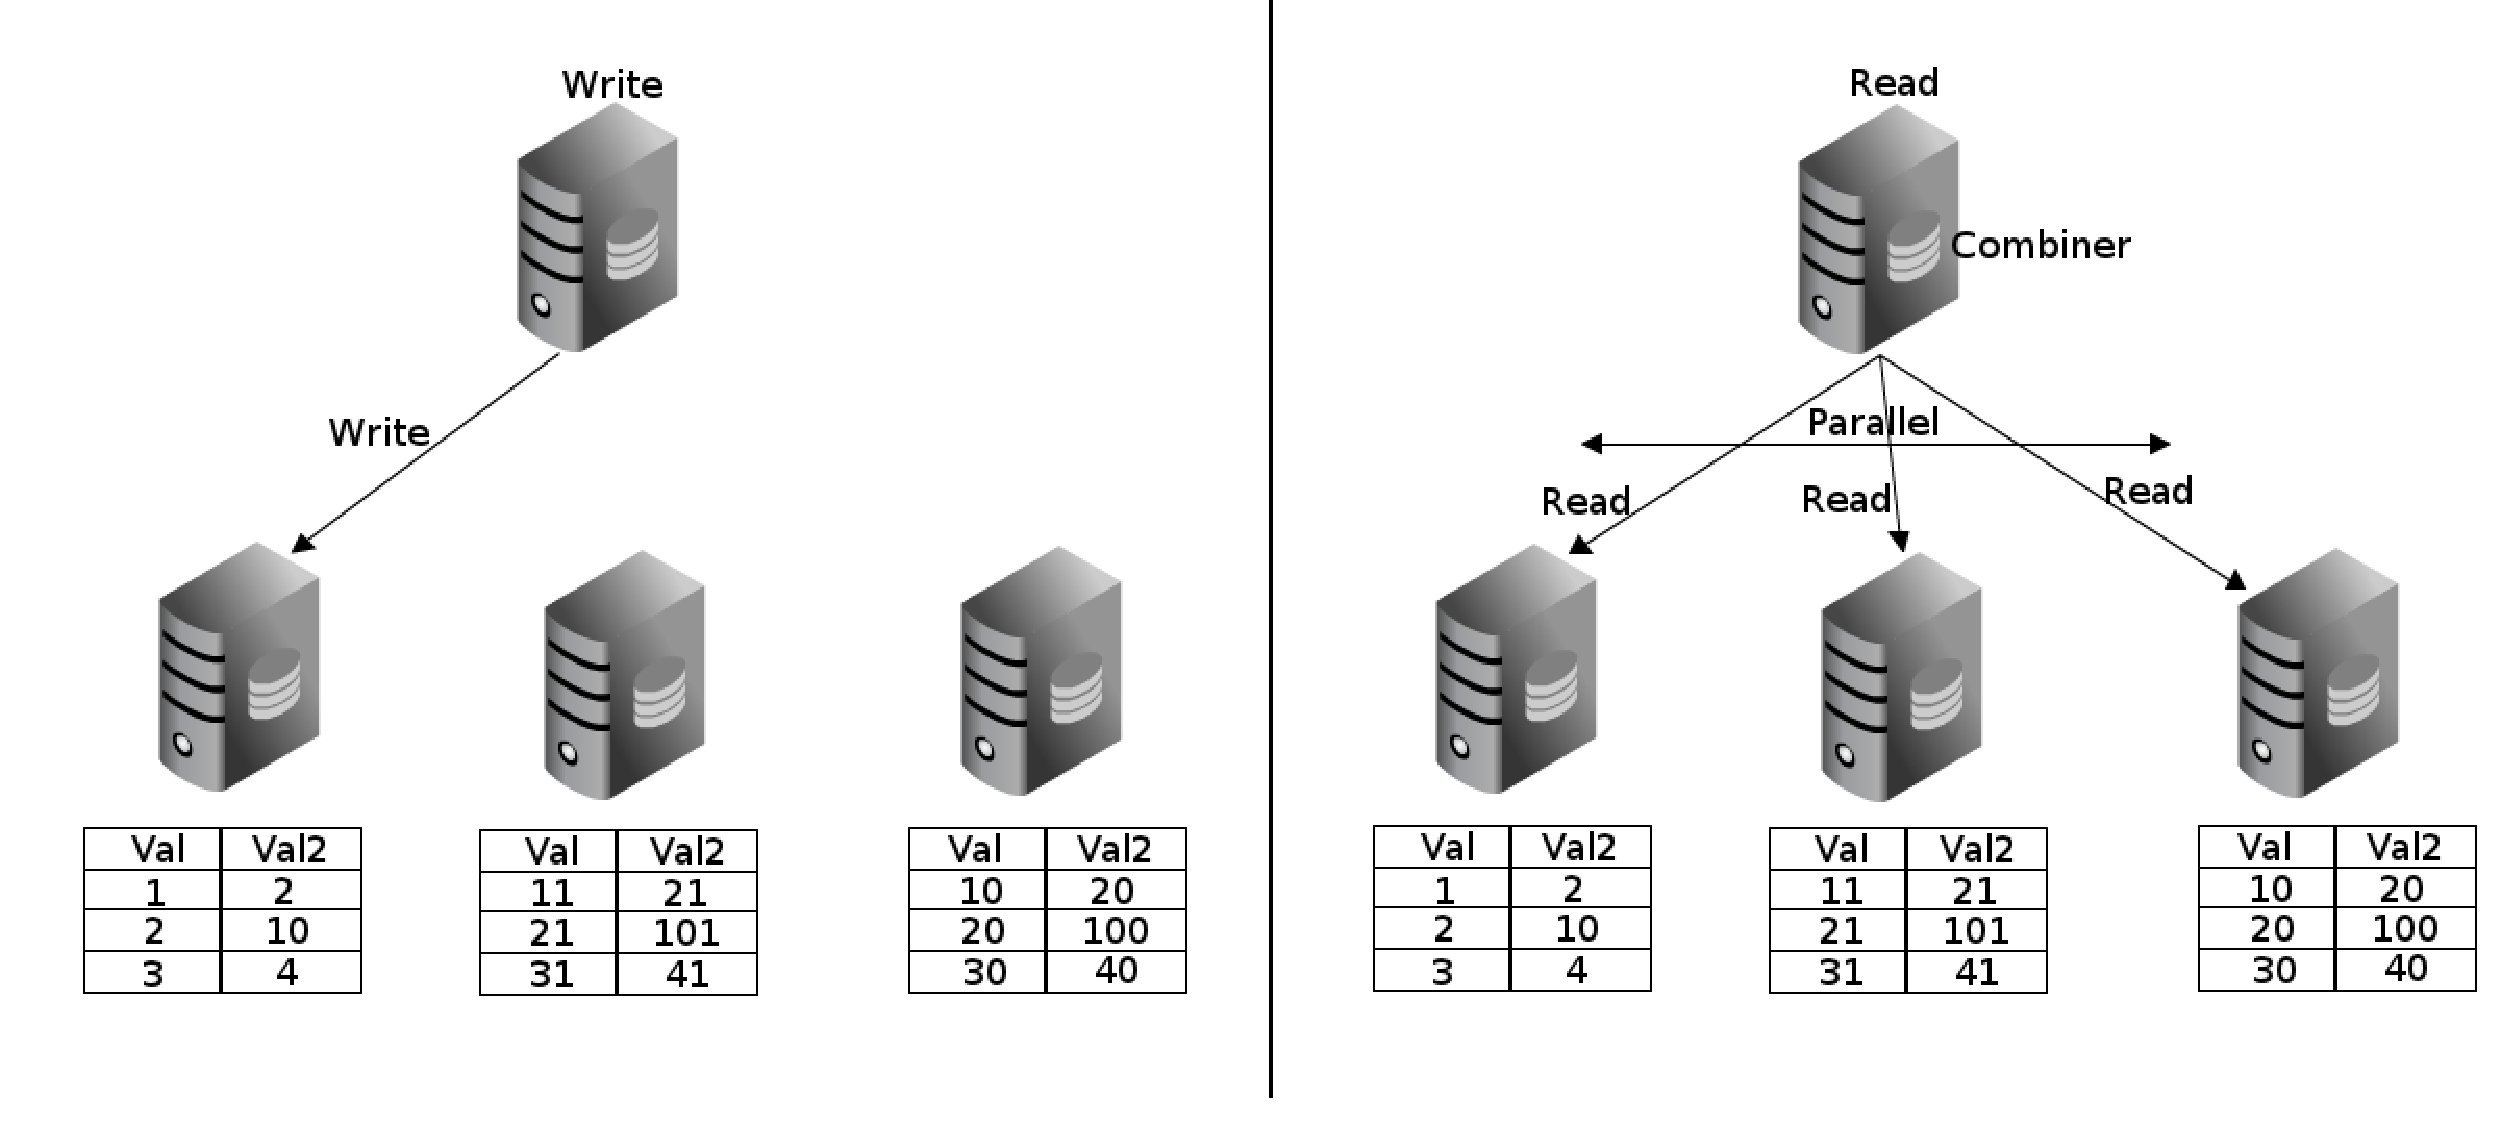
\includegraphics[width=1\textwidth]{postgres-x2-02.pdf}}
  \caption{Распределенные таблицы}
  \label{fig:postgres-x22}
\end{figure}

\begin{figure}[ht!]
  \center{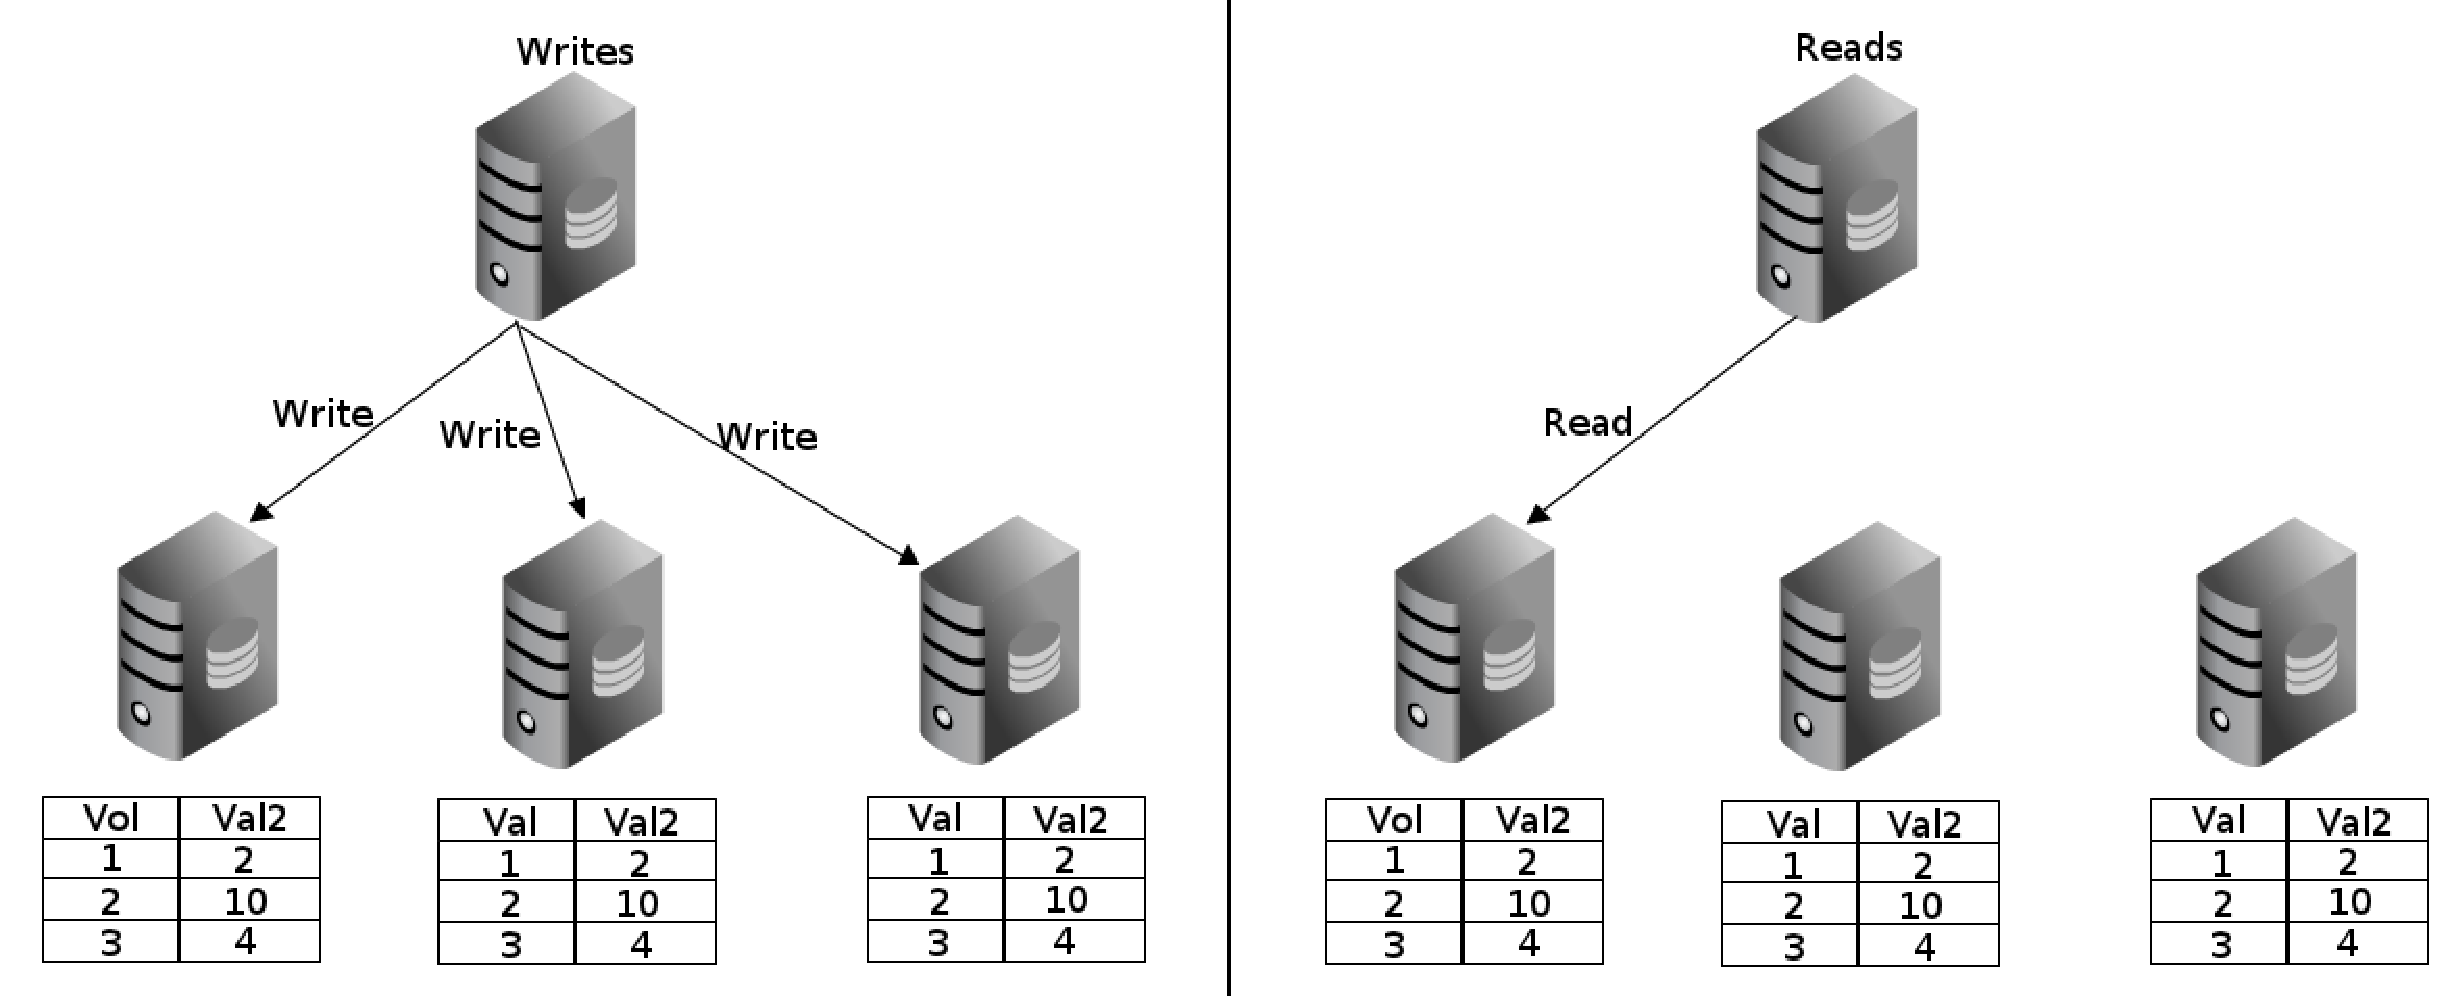
\includegraphics[width=1\textwidth]{postgres-x2-03.pdf}}
  \caption{Реплицированные таблицы}
  \label{fig:postgres-x23}
\end{figure}

\begin{enumerate}
  \item Распределенные таблицы (distributed tables, рис.~\ref{fig:postgres-x22}): данные по таблице распределяются на указанный набор обработчиков данных с использованием указанной стратегии (hash, round-robin, modulo). Каждая запись в таблице находится только на одном обработчике данных. Параллельно могут быть записаны или прочитаны данные с различных обработчиков данных. За счет этого значительно улучшена производительность на запись и чтение;
  \item Реплицированные таблицы (replicated tables, рис.~\ref{fig:postgres-x23}): данные по таблице реплицируется (клонируются) на указанный набор обработчиков данных. Каждая запись в таблице находится на всех обработчиках данных (которые были указаны) и любые изменения дублируются на все обработчики данных. Так как все данные доступны на любом обработчике данных, координатор может собрать все данные из одного узла, что позволяет направить различные запросы на различные обработчики данных. Таким образом создается балансировка нагрузки и увеличения пропускной способности на чтение.
\end{enumerate}

\subsection{Таблицы и запросы к ним}

После установки работа с Postgres-X2 ведется как с обыкновенным PostgreSQL. Подключаться для работы с данными нужно только к координаторам (по умолчанию координатор работает на порту 5432). Для начала создадим распределенные таблицы.

\begin{lstlisting}[language=SQL,label=lst:postgres-x22,caption=Создание распределенных таблиц]
CREATE TABLE
users_with_hash (id SERIAL, type INT, ...)
DISTRIBUTE by HASH(id);

CREATE TABLE
users_with_modulo (id SERIAL, type INT, ...)
DISTRIBUTE by MODULO(id);

CREATE TABLE
users_with_rrobin (id SERIAL, type INT, ...)
DISTRIBUTE by ROUNDROBIN;
\end{lstlisting}

На листинге~\ref{lst:postgres-x22} создано 3 распределенные таблицы:

\begin{enumerate}
  \item Таблица \lstinline!users_with_hash! распределяется по хешу значения из указанного поля в таблице (тут указано поле id) по обработчикам данных. Вот как распределились первые 15 значений:

\begin{lstlisting}[language=SQL,label=lst:postgres-x23,caption=Данные с координатора и обработчиков данных]
# координатор
$ psql
# SELECT id, type from users_with_hash ORDER BY id;
 id   | type
-------+-------
     1 |   946
     2 |   153
     3 |   484
     4 |   422
     5 |   785
     6 |   906
     7 |   973
     8 |   699
     9 |   434
    10 |   986
    11 |   135
    12 |  1012
    13 |   395
    14 |   667
    15 |   324

# первый обработчик данных
$ psql -p15432
# SELECT id, type from users_with_hash ORDER BY id;
  id  | type
------+-------
    1 |   946
    2 |   153
    5 |   785
    6 |   906
    8 |   699
    9 |   434
   12 |  1012
   13 |   395
   15 |   324

# второй обработчик данных
$ psql -p15433
# SELECT id, type from users_with_hash ORDER BY id;
 id   | type
-------+-------
     3 |   484
     4 |   422
     7 |   973
    10 |   986
    11 |   135
    14 |   667
\end{lstlisting}

  \item Таблица \lstinline!users_with_modulo! распределяется по модулю значения из указанного поля в таблице (тут указано поле id) по обработчикам данных. Вот как распределились первые 15 значений:

\begin{lstlisting}[language=SQL,label=lst:postgres-x24,caption=Данные с координатора и обработчиков данных]
# координатор
$ psql
# SELECT id, type from users_with_modulo ORDER BY id;
 id   | type
-------+-------
     1 |   883
     2 |   719
     3 |    29
     4 |   638
     5 |   363
     6 |   946
     7 |   440
     8 |   331
     9 |   884
    10 |   199
    11 |    78
    12 |   791
    13 |   345
    14 |   476
    15 |   860

# первый обработчик данных
$ psql -p15432
# SELECT id, type from users_with_modulo ORDER BY id;
  id   | type
-------+-------
     2 |   719
     4 |   638
     6 |   946
     8 |   331
    10 |   199
    12 |   791
    14 |   476

# второй обработчик данных
$ psql -p15433
# SELECT id, type from users_with_modulo ORDER BY id;
  id  | type
------+-------
    1 |   883
    3 |    29
    5 |   363
    7 |   440
    9 |   884
   11 |    78
   13 |   345
   15 |   860
\end{lstlisting}

  \item Таблица \lstinline!users_with_rrobin! распределяется циклическим способом(round-robin) по обработчикам данных. Вот как распределились первые 15 значений:

\begin{lstlisting}[language=SQL,label=lst:postgres-x25,caption=Данные с координатора и обработчиков данных]
# координатор
$ psql
# SELECT id, type from users_with_rrobin ORDER BY id;
 id   | type
-------+-------
     1 |   890
     2 |   198
     3 |   815
     4 |   446
     5 |    61
     6 |   337
     7 |   948
     8 |   446
     9 |   796
    10 |   422
    11 |   242
    12 |   795
    13 |   314
    14 |   240
    15 |   733

# первый обработчик данных
$ psql -p15432
# SELECT id, type from users_with_rrobin ORDER BY id;
  id   | type
-------+-------
     2 |   198
     4 |   446
     6 |   337
     8 |   446
    10 |   422
    12 |   795
    14 |   240

# второй обработчик данных
$ psql -p15433
# SELECT id, type from users_with_rrobin ORDER BY id;
  id  | type
------+-------
    1 |   890
    3 |   815
    5 |    61
    7 |   948
    9 |   796
   11 |   242
   13 |   314
   15 |   733
\end{lstlisting}

\end{enumerate}

Теперь создадим реплицированную таблицу:

\begin{lstlisting}[language=SQL,label=lst:postgres-x220,caption=Создание реплицированной таблицы]
CREATE TABLE
users_replicated (id SERIAL, type INT, ...)
DISTRIBUTE by REPLICATION;
\end{lstlisting}

Естественно данные идентичны на всех обработчиках данных:

\begin{lstlisting}[language=SQL,label=lst:postgres-x221,caption=Данные с координатора и обработчиков данных]
# SELECT id, type from users_replicated  ORDER BY id;
  id   | type
-------+-------
     1 |    75
     2 |   262
     3 |   458
     4 |   779
     5 |   357
     6 |    51
     7 |   249
     8 |   444
     9 |   890
    10 |   810
    11 |   809
    12 |   166
    13 |   605
    14 |   401
    15 |    58
\end{lstlisting}

Рассмотрим как выполняются запросы для таблиц. Выберем все записи из распределенной таблицы:

\begin{lstlisting}[language=SQL,label=lst:postgres-x26,caption=Выборка записей из распределенной таблицы]
# EXPLAIN VERBOSE SELECT * from users_with_modulo ORDER BY id;
                                      QUERY PLAN
--------------------------------------------------------------------------------------
 Sort  (cost=49.83..52.33 rows=1000 width=8)
   Output: id, type
   Sort Key: users_with_modulo.id
   ->  Result  (cost=0.00..0.00 rows=1000 width=8)
         Output: id, type
         ->  Data Node Scan on users_with_modulo  (cost=0.00..0.00 rows=1000 width=8)
               Output: id, type
               Node/s: dn1, dn2
               Remote query: SELECT id, type FROM ONLY users_with_modulo WHERE true
(9 rows)
\end{lstlisting}

Как видно на листинге~\ref{lst:postgres-x26} координатор собирает данные из обработчиков данных, а потом собирает их вместе.

Подсчет суммы с группировкой по полю из распределенной таблицы:

\begin{lstlisting}[language=SQL,label=lst:postgres-x27,caption=Выборка записей из распределенной таблицы]
# EXPLAIN VERBOSE SELECT sum(id) from users_with_modulo GROUP BY type;
                                                                      QUERY PLAN
------------------------------------------------------------------------------------------------------------------------------------------------------
 HashAggregate  (cost=5.00..5.01 rows=1 width=8)
   Output: pg_catalog.sum((sum(users_with_modulo.id))), users_with_modulo.type
   ->  Materialize  (cost=0.00..0.00 rows=0 width=0)
         Output: (sum(users_with_modulo.id)), users_with_modulo.type
         ->  Data Node Scan on "__REMOTE_GROUP_QUERY__"  (cost=0.00..0.00 rows=1000 width=8)
               Output: sum(users_with_modulo.id), users_with_modulo.type
               Node/s: dn1, dn2
               Remote query: SELECT sum(group_1.id), group_1.type  FROM (SELECT id, type FROM ONLY users_with_modulo WHERE true) group_1 GROUP BY 2
(8 rows)
\end{lstlisting}

JOIN между и с участием реплицированных таблиц, а также JOIN между распределенными по одному и тому же полю в таблицах будет выполняются на обработчиках данных. Но JOIN с участием распределенных таблиц по другим ключам будут выполнены на координаторе и скорее всего это будет медленно (листинг~\ref{lst:postgres-x28}).

\begin{lstlisting}[language=SQL,label=lst:postgres-x28,caption=Выборка записей из распределенной таблицы]
# EXPLAIN VERBOSE SELECT * from users_with_modulo, users_with_hash WHERE users_with_modulo.id = users_with_hash.id;
                                            QUERY PLAN
--------------------------------------------------------------------------------------------------
 Nested Loop  (cost=0.00..0.01 rows=1 width=16)
   Output: users_with_modulo.id, users_with_modulo.type, users_with_hash.id, users_with_hash.type
   Join Filter: (users_with_modulo.id = users_with_hash.id)
   ->  Data Node Scan on users_with_modulo  (cost=0.00..0.00 rows=1000 width=8)
         Output: users_with_modulo.id, users_with_modulo.type
         Node/s: dn1, dn2
         Remote query: SELECT id, type FROM ONLY users_with_modulo WHERE true
   ->  Data Node Scan on users_with_hash  (cost=0.00..0.00 rows=1000 width=8)
         Output: users_with_hash.id, users_with_hash.type
         Node/s: dn1, dn2
         Remote query: SELECT id, type FROM ONLY users_with_hash WHERE true
(11 rows)
\end{lstlisting}

Пример выборки данных из реплицированной таблицы:

\begin{lstlisting}[language=SQL,label=lst:postgres-x222,caption=Выборка записей из реплицированной таблицы]
# EXPLAIN VERBOSE SELECT * from users_replicated;
                                 QUERY PLAN
----------------------------------------------------------------------------
 Data Node Scan on "__REMOTE_FQS_QUERY__"  (cost=0.00..0.00 rows=0 width=0)
   Output: users_replicated.id, users_replicated.type
   Node/s: dn1
   Remote query: SELECT id, type FROM users_replicated
(4 rows)
\end{lstlisting}

Как видно из запроса для выборки данных используется один обработчик данных, а не все (что и логично).

\subsection{Высокая доступность (HA)}

По архитектуре у Postgres-X2 всегда есть согласованность данных. По \href{http://en.wikipedia.org/wiki/CAP\_theorem}{теореме CAP} в такой системе тяжело обеспечить высокую доступность. Для достижения высокой доступности в распределенных системах требуется избыточность данных, резервные копии и автоматическое восстановление. В Postgres-X2 избыточность данных может быть достигнута с помощью PostgreSQL потоковой (streaming) репликации с hot-standby для обработчиков данных. Каждый координатор способен записывать и читать данные независимо от другого, поэтому координаторы способны заменять друг друга. Поскольку GTM отдельный процесс и может стать точкой отказа, лучше создать GTM-standby как резервную копию. Ну а вот для автоматического восстановления придется использовать сторонние утилиты.

\subsection{Ограничения}

\begin{enumerate}
  \item Postgres-X2 базируется на PostgreSQL 9.3;
  \item Нет системы репартиционирования при добавлении или удалении нод (в разработке);
  \item Нет глобальных \lstinline!UNIQUE! на распределенных таблицах;
  \item Не поддерживаются foreign keys между нодами поскольку такой ключ должен вести на данные расположенные на том же обработчике данных;
  \item Не поддерживаются курсоры (в разработке);
  \item Не поддерживается \lstinline!INSERT ... RETURNING! (в разработке);
  \item Невозможно удаление и добавление нод в кластер без полной реинициализации кластера (в разработке).
\end{enumerate}

\subsection{Заключение}

Postgres-X2 очень перспективное решение для создание кластера на основе PostgreSQL. И хоть это решение имеет ряд недостатков, нестабильно (очень часты случаи падения координаторов при тяжелых запросах) и еще очень молодое, со временем это решение может стать стандартом для масштабирования систем на PostgreSQL.